\documentclass{article}\usepackage{graphicx}\usepackage{placeins}\usepackage{tikz}\begin{document}

\FloatBarrier
\begin{figure}[!htb]\centering
\begin{minipage}[b]{.99\textwidth}\begin{verbatim}
./adjacencyMatrix.py [or ./tikzGraph.py] \
    "4" "d" "-" \
    "char" "ex1" "directed clique" \
    "list" "1,1,1,1,1,1,1,1,1,1,1,1" ["circle"]

\end{verbatim}\end{minipage}
\begin{minipage}[b]{.49\textwidth} \resizebox {1.0\textwidth} {!} {
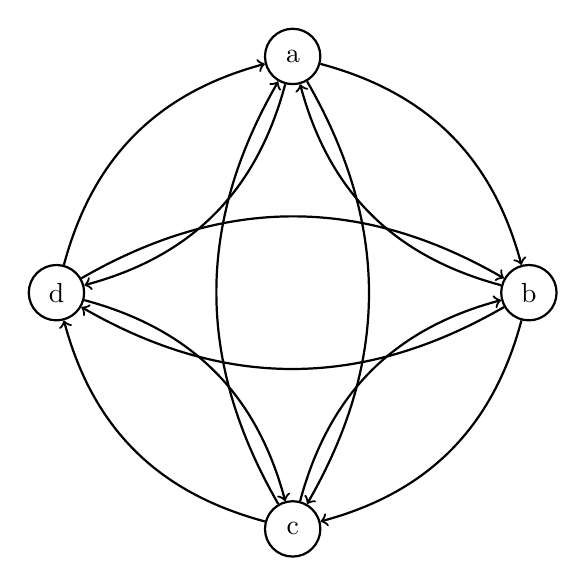
\begin{tikzpicture}
\usetikzlibrary{arrows}
\tikzset{edge/.style = {->, thick}}
\tikzset{vertex/.style = {shape=circle, draw, thick, minimum size=2em}}
\def \n {4}
\def \radius {3cm}
\node[vertex](v0) at (90:\radius) {a};
\node[vertex](v1) at (0:\radius) {b};
\node[vertex](v2) at (270:\radius) {c};
\node[vertex](v3) at (180:\radius) {d};
\draw[edge] (v0) to[bend left] (v1);
\draw[edge] (v0) to[bend left] (v2);
\draw[edge] (v0) to[bend left] (v3);
\draw[edge] (v1) to[bend left] (v0);
\draw[edge] (v1) to[bend left] (v2);
\draw[edge] (v1) to[bend left] (v3);
\draw[edge] (v2) to[bend left] (v0);
\draw[edge] (v2) to[bend left] (v1);
\draw[edge] (v2) to[bend left] (v3);
\draw[edge] (v3) to[bend left] (v0);
\draw[edge] (v3) to[bend left] (v1);
\draw[edge] (v3) to[bend left] (v2);
\end{tikzpicture}
} \caption{directed clique} \label{fig:ex1} \end{minipage}
\hfill
\begin{minipage}[b]{.49\textwidth} \resizebox {1.0\textwidth} {!} {
\begin{tabular}{r|cccc}
	&	a	&	b	&	c	&	d	\\
\hline
a	&	-	&	1	&	1	&	1	\\
b	&	1	&	-	&	1	&	1	\\
c	&	1	&	1	&	-	&	1	\\
d	&	1	&	1	&	1	&	-	\\
\end{tabular}
} \caption{directed clique} \label{tab:ex1} \end{minipage}
\end{figure}

\FloatBarrier
\begin{figure}[!htb]\centering
\begin{minipage}[b]{.99\textwidth}\begin{verbatim}
./adjacencyMatrix.py [or ./tikzGraph.py] \
    "6" "d" "-" \
    "char" "ex2" "directed ring" \
    "list" "1,0,0,0,0,0,1,0,0,0,0,0,1,0,0,0,0,0,1,0,0,0,0,0,1,1,0,0,0,0" ["circle"]

\end{verbatim}\end{minipage}
\begin{minipage}[b]{.49\textwidth} \resizebox {1.0\textwidth} {!} {
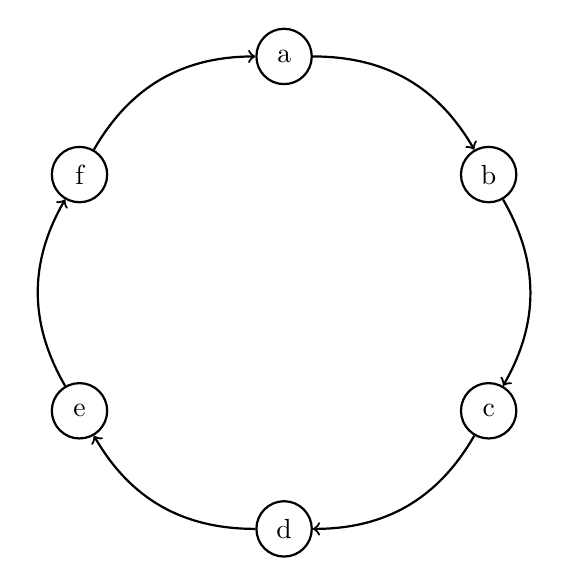
\begin{tikzpicture}
\usetikzlibrary{arrows}
\tikzset{edge/.style = {->, thick}}
\tikzset{vertex/.style = {shape=circle, draw, thick, minimum size=2em}}
\def \n {6}
\def \radius {3cm}
\node[vertex](v0) at (90:\radius) {a};
\node[vertex](v1) at (30:\radius) {b};
\node[vertex](v2) at (330:\radius) {c};
\node[vertex](v3) at (270:\radius) {d};
\node[vertex](v4) at (210:\radius) {e};
\node[vertex](v5) at (150:\radius) {f};
\draw[edge] (v0) to[bend left] (v1);
\draw[edge] (v1) to[bend left] (v2);
\draw[edge] (v2) to[bend left] (v3);
\draw[edge] (v3) to[bend left] (v4);
\draw[edge] (v4) to[bend left] (v5);
\draw[edge] (v5) to[bend left] (v0);
\end{tikzpicture}
} \caption{directed ring} \label{fig:ex2} \end{minipage}
\hfill
\begin{minipage}[b]{.49\textwidth} \resizebox {1.0\textwidth} {!} {
\begin{tabular}{r|cccccc}
	&	a	&	b	&	c	&	d	&	e	&	f	\\
\hline
a	&	-	&	1	&	0	&	0	&	0	&	0	\\
b	&	0	&	-	&	1	&	0	&	0	&	0	\\
c	&	0	&	0	&	-	&	1	&	0	&	0	\\
d	&	0	&	0	&	0	&	-	&	1	&	0	\\
e	&	0	&	0	&	0	&	0	&	-	&	1	\\
f	&	1	&	0	&	0	&	0	&	0	&	-	\\
\end{tabular}
} \caption{directed ring} \label{tab:ex2} \end{minipage}
\end{figure}

\FloatBarrier
\begin{figure}[!htb]\centering
\begin{minipage}[b]{.99\textwidth}\begin{verbatim}
./adjacencyMatrix.py [or ./tikzGraph.py] \
    "4" "u" "-" \
    "char" "ex3" "undirected clique" \
    "list" "1,1,1,1,1,1" ["circle"]

\end{verbatim}\end{minipage}
\begin{minipage}[b]{.49\textwidth} \resizebox {1.0\textwidth} {!} {
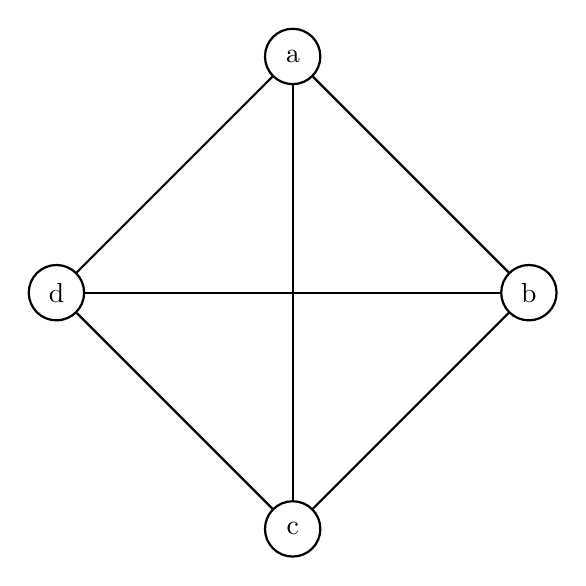
\begin{tikzpicture}
\usetikzlibrary{arrows}
\tikzset{edge/.style = {-, thick}}
\tikzset{vertex/.style = {shape=circle, draw, thick, minimum size=2em}}
\def \n {4}
\def \radius {3cm}
\node[vertex](v0) at (90:\radius) {a};
\node[vertex](v1) at (0:\radius) {b};
\node[vertex](v2) at (270:\radius) {c};
\node[vertex](v3) at (180:\radius) {d};
\draw[edge] (v0) to (v1);
\draw[edge] (v0) to (v2);
\draw[edge] (v0) to (v3);
\draw[edge] (v1) to (v2);
\draw[edge] (v1) to (v3);
\draw[edge] (v2) to (v3);
\end{tikzpicture}
} \caption{undirected clique} \label{fig:ex3} \end{minipage}
\hfill
\begin{minipage}[b]{.49\textwidth} \resizebox {1.0\textwidth} {!} {
\begin{tabular}{r|cccc}
	&	a	&	b	&	c	&	d	\\
\hline
a	&	-	&	1	&	1	&	1	\\
b	&		&	-	&	1	&	1	\\
c	&		&		&	-	&	1	\\
d	&		&		&		&	-	\\
\end{tabular}
} \caption{undirected clique} \label{tab:ex3} \end{minipage}
\end{figure}

\FloatBarrier
\begin{figure}[!htb]\centering
\begin{minipage}[b]{.99\textwidth}\begin{verbatim}
./adjacencyMatrix.py [or ./tikzGraph.py] \
    "6" "u" "-" \
    "char" "ex4" "undirected ring" \
    "list" "1,0,0,0,1,1,0,0,0,1,0,0,1,0,1" ["circle"]

\end{verbatim}\end{minipage}
\begin{minipage}[b]{.49\textwidth} \resizebox {1.0\textwidth} {!} {
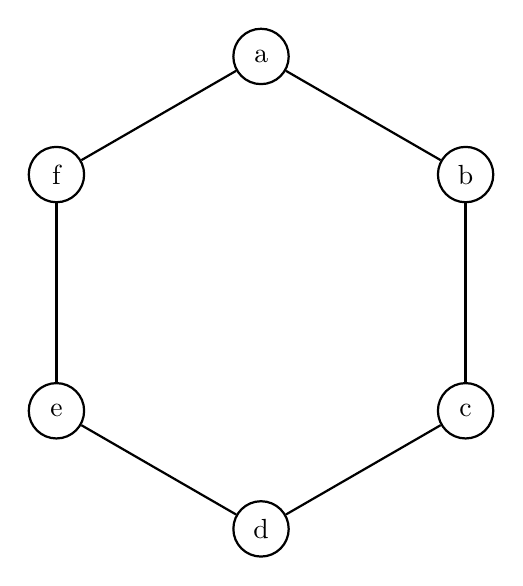
\begin{tikzpicture}
\usetikzlibrary{arrows}
\tikzset{edge/.style = {-, thick}}
\tikzset{vertex/.style = {shape=circle, draw, thick, minimum size=2em}}
\def \n {6}
\def \radius {3cm}
\node[vertex](v0) at (90:\radius) {a};
\node[vertex](v1) at (30:\radius) {b};
\node[vertex](v2) at (330:\radius) {c};
\node[vertex](v3) at (270:\radius) {d};
\node[vertex](v4) at (210:\radius) {e};
\node[vertex](v5) at (150:\radius) {f};
\draw[edge] (v0) to (v1);
\draw[edge] (v0) to (v5);
\draw[edge] (v1) to (v2);
\draw[edge] (v2) to (v3);
\draw[edge] (v3) to (v4);
\draw[edge] (v4) to (v5);
\end{tikzpicture}
} \caption{undirected ring} \label{fig:ex4} \end{minipage}
\hfill
\begin{minipage}[b]{.49\textwidth} \resizebox {1.0\textwidth} {!} {
\begin{tabular}{r|cccccc}
	&	a	&	b	&	c	&	d	&	e	&	f	\\
\hline
a	&	-	&	1	&	0	&	0	&	0	&	1	\\
b	&		&	-	&	1	&	0	&	0	&	0	\\
c	&		&		&	-	&	1	&	0	&	0	\\
d	&		&		&		&	-	&	1	&	0	\\
e	&		&		&		&		&	-	&	1	\\
f	&		&		&		&		&		&	-	\\
\end{tabular}
} \caption{undirected ring} \label{tab:ex4} \end{minipage}
\end{figure}

\FloatBarrier
\begin{figure}[!htb]\centering
\begin{minipage}[b]{.99\textwidth}\begin{verbatim}
./adjacencyMatrix.py [or ./tikzGraph.py] \
    "5" "u" "-" \
    "index" "ex5" "undirected pentagram" \
    "list" "1,1,1,1,1,1,1,1,1,1" ["circle"]

\end{verbatim}\end{minipage}
\begin{minipage}[b]{.49\textwidth} \resizebox {1.0\textwidth} {!} {
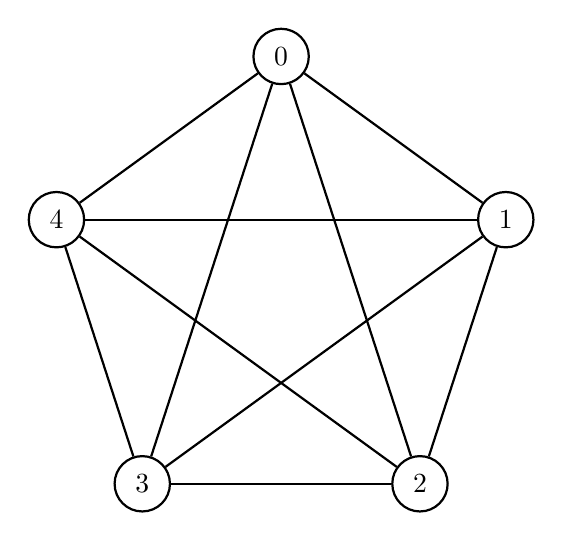
\begin{tikzpicture}
\usetikzlibrary{arrows}
\tikzset{edge/.style = {-, thick}}
\tikzset{vertex/.style = {shape=circle, draw, thick, minimum size=2em}}
\def \n {5}
\def \radius {3cm}
\node[vertex](v0) at (90:\radius) {0};
\node[vertex](v1) at (18:\radius) {1};
\node[vertex](v2) at (306:\radius) {2};
\node[vertex](v3) at (234:\radius) {3};
\node[vertex](v4) at (162:\radius) {4};
\draw[edge] (v0) to (v1);
\draw[edge] (v0) to (v2);
\draw[edge] (v0) to (v3);
\draw[edge] (v0) to (v4);
\draw[edge] (v1) to (v2);
\draw[edge] (v1) to (v3);
\draw[edge] (v1) to (v4);
\draw[edge] (v2) to (v3);
\draw[edge] (v2) to (v4);
\draw[edge] (v3) to (v4);
\end{tikzpicture}
} \caption{undirected pentagram} \label{fig:ex5} \end{minipage}
\hfill
\begin{minipage}[b]{.49\textwidth} \resizebox {1.0\textwidth} {!} {
\begin{tabular}{r|ccccc}
	&	0	&	1	&	2	&	3	&	4	\\
\hline
0	&	-	&	1	&	1	&	1	&	1	\\
1	&		&	-	&	1	&	1	&	1	\\
2	&		&		&	-	&	1	&	1	\\
3	&		&		&		&	-	&	1	\\
4	&		&		&		&		&	-	\\
\end{tabular}
} \caption{undirected pentagram} \label{tab:ex5} \end{minipage}
\end{figure}

\FloatBarrier
\begin{figure}[!htb]\centering
\begin{minipage}[b]{.99\textwidth}\begin{verbatim}
./adjacencyMatrix.py [or ./tikzGraph.py] \
    "12" "u" "-" \
    "index" "ex6" "undirected clock" \
    "list" "1,1,1,1,1,1,1,1,1,1,1,1,1,1,1,1,1,1,1,1,1,1,1,1,1,1,1,1,1,1,1,1,1,1,1,1,1,1,1,1,1,1,1,1,1,1,1,1,1,1,1,1,1,1,1,1,1,1,1,1,1,1,1,1,1,1" ["circle"]

\end{verbatim}\end{minipage}
\begin{minipage}[b]{.49\textwidth} \resizebox {1.0\textwidth} {!} {
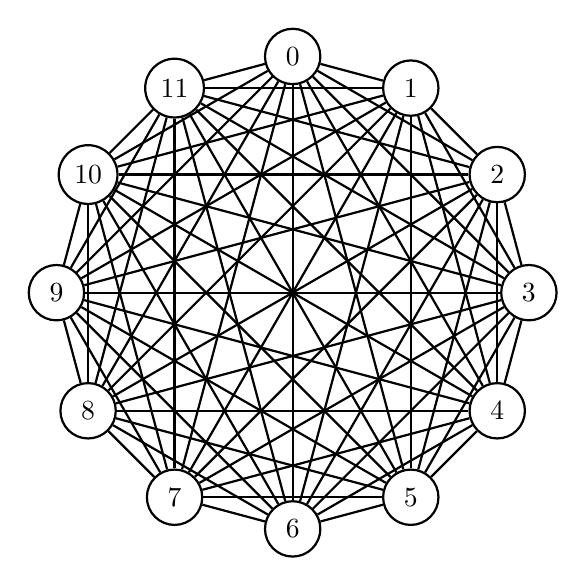
\begin{tikzpicture}
\usetikzlibrary{arrows}
\tikzset{edge/.style = {-, thick}}
\tikzset{vertex/.style = {shape=circle, draw, thick, minimum size=2em}}
\def \n {12}
\def \radius {3cm}
\node[vertex](v0) at (90:\radius) {0};
\node[vertex](v1) at (60:\radius) {1};
\node[vertex](v2) at (30:\radius) {2};
\node[vertex](v3) at (0:\radius) {3};
\node[vertex](v4) at (330:\radius) {4};
\node[vertex](v5) at (300:\radius) {5};
\node[vertex](v6) at (270:\radius) {6};
\node[vertex](v7) at (240:\radius) {7};
\node[vertex](v8) at (210:\radius) {8};
\node[vertex](v9) at (180:\radius) {9};
\node[vertex](v10) at (150:\radius) {10};
\node[vertex](v11) at (120:\radius) {11};
\draw[edge] (v0) to (v1);
\draw[edge] (v0) to (v2);
\draw[edge] (v0) to (v3);
\draw[edge] (v0) to (v4);
\draw[edge] (v0) to (v5);
\draw[edge] (v0) to (v6);
\draw[edge] (v0) to (v7);
\draw[edge] (v0) to (v8);
\draw[edge] (v0) to (v9);
\draw[edge] (v0) to (v10);
\draw[edge] (v0) to (v11);
\draw[edge] (v1) to (v2);
\draw[edge] (v1) to (v3);
\draw[edge] (v1) to (v4);
\draw[edge] (v1) to (v5);
\draw[edge] (v1) to (v6);
\draw[edge] (v1) to (v7);
\draw[edge] (v1) to (v8);
\draw[edge] (v1) to (v9);
\draw[edge] (v1) to (v10);
\draw[edge] (v1) to (v11);
\draw[edge] (v2) to (v3);
\draw[edge] (v2) to (v4);
\draw[edge] (v2) to (v5);
\draw[edge] (v2) to (v6);
\draw[edge] (v2) to (v7);
\draw[edge] (v2) to (v8);
\draw[edge] (v2) to (v9);
\draw[edge] (v2) to (v10);
\draw[edge] (v2) to (v11);
\draw[edge] (v3) to (v4);
\draw[edge] (v3) to (v5);
\draw[edge] (v3) to (v6);
\draw[edge] (v3) to (v7);
\draw[edge] (v3) to (v8);
\draw[edge] (v3) to (v9);
\draw[edge] (v3) to (v10);
\draw[edge] (v3) to (v11);
\draw[edge] (v4) to (v5);
\draw[edge] (v4) to (v6);
\draw[edge] (v4) to (v7);
\draw[edge] (v4) to (v8);
\draw[edge] (v4) to (v9);
\draw[edge] (v4) to (v10);
\draw[edge] (v4) to (v11);
\draw[edge] (v5) to (v6);
\draw[edge] (v5) to (v7);
\draw[edge] (v5) to (v8);
\draw[edge] (v5) to (v9);
\draw[edge] (v5) to (v10);
\draw[edge] (v5) to (v11);
\draw[edge] (v6) to (v7);
\draw[edge] (v6) to (v8);
\draw[edge] (v6) to (v9);
\draw[edge] (v6) to (v10);
\draw[edge] (v6) to (v11);
\draw[edge] (v7) to (v8);
\draw[edge] (v7) to (v9);
\draw[edge] (v7) to (v10);
\draw[edge] (v7) to (v11);
\draw[edge] (v8) to (v9);
\draw[edge] (v8) to (v10);
\draw[edge] (v8) to (v11);
\draw[edge] (v9) to (v10);
\draw[edge] (v9) to (v11);
\draw[edge] (v10) to (v11);
\end{tikzpicture}
} \caption{undirected clock} \label{fig:ex6} \end{minipage}
\hfill
\begin{minipage}[b]{.49\textwidth} \resizebox {1.0\textwidth} {!} {
\begin{tabular}{r|cccccccccccc}
	&	0	&	1	&	2	&	3	&	4	&	5	&	6	&	7	&	8	&	9	&	10	&	11	\\
\hline
0	&	-	&	1	&	1	&	1	&	1	&	1	&	1	&	1	&	1	&	1	&	1	&	1	\\
1	&		&	-	&	1	&	1	&	1	&	1	&	1	&	1	&	1	&	1	&	1	&	1	\\
2	&		&		&	-	&	1	&	1	&	1	&	1	&	1	&	1	&	1	&	1	&	1	\\
3	&		&		&		&	-	&	1	&	1	&	1	&	1	&	1	&	1	&	1	&	1	\\
4	&		&		&		&		&	-	&	1	&	1	&	1	&	1	&	1	&	1	&	1	\\
5	&		&		&		&		&		&	-	&	1	&	1	&	1	&	1	&	1	&	1	\\
6	&		&		&		&		&		&		&	-	&	1	&	1	&	1	&	1	&	1	\\
7	&		&		&		&		&		&		&		&	-	&	1	&	1	&	1	&	1	\\
8	&		&		&		&		&		&		&		&		&	-	&	1	&	1	&	1	\\
9	&		&		&		&		&		&		&		&		&		&	-	&	1	&	1	\\
10	&		&		&		&		&		&		&		&		&		&		&	-	&	1	\\
11	&		&		&		&		&		&		&		&		&		&		&		&	-	\\
\end{tabular}
} \caption{undirected clock} \label{tab:ex6} \end{minipage}
\end{figure}
\end{document}
